% CAPITULO 1: ONBOARDING (VERSION SIMPLIFICADA)

\chapter{Onboarding e Identidad}
\label{ch:onboarding}

Todo nodo en \sdc{} debe tener una identidad unica para garantizar la auditoria.

\section{Configuracion de Identidad}
\label{sec:config-identidad}

Al iniciar la aplicacion, el sistema solicita configuracion basica de identidad.

\begin{figure}[H]
\centering
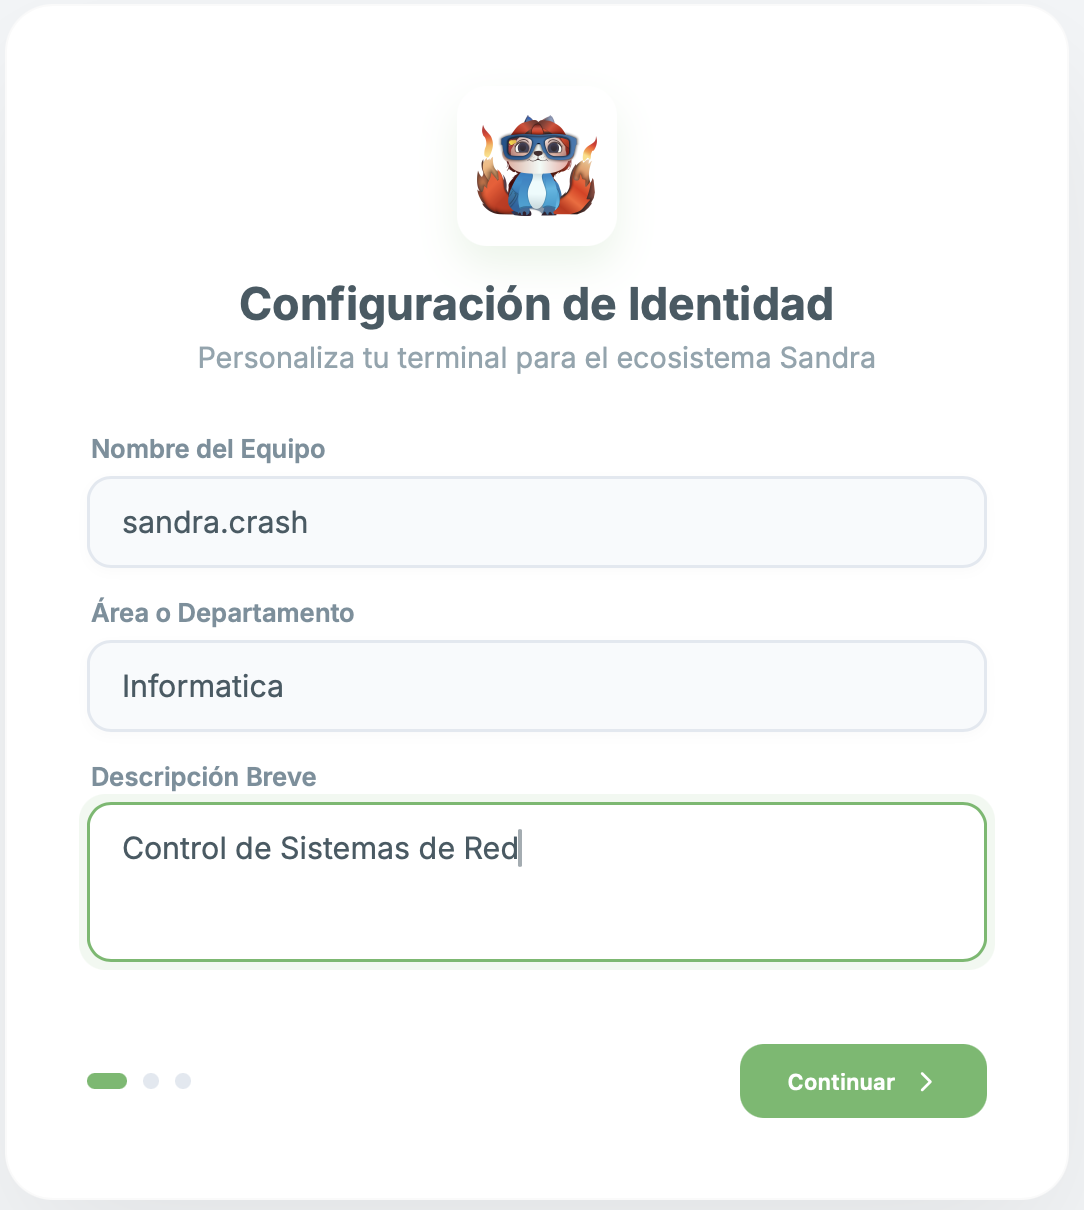
\includegraphics[width=0.3\textwidth]{anexos/2 config.png}
\caption{Pantalla de configuracion inicial}
\label{fig:config-inicial}
\end{figure}

\subsection{Campos de Configuracion}

\begin{table}[H]
\centering
\begin{tabular}{p{3cm}p{3cm}p{5cm}}
\toprule
\textbf{Campo} & \textbf{Ejemplo} & \textbf{Descripcion} \\
\midrule
Nombre del Equipo & sandra.crash & Identificador unico \\
Area & Desarrollo & Departamento \\
\bottomrule
\end{tabular}
\caption{Campos de configuracion}
\label{tab:campos-identidad}
\end{table}

\begin{warnbox}[Importancia del Nombre]
Asigna nombres descriptivos. Estos apareceran en los logs del Monitor.
\end{warnbox}

\section{Vinculacion del Nodo}
\label{sec:vinculacion}

SDC detecta automaticamente el entorno y genera un Client ID unico.

\begin{figure}[H]
\centering
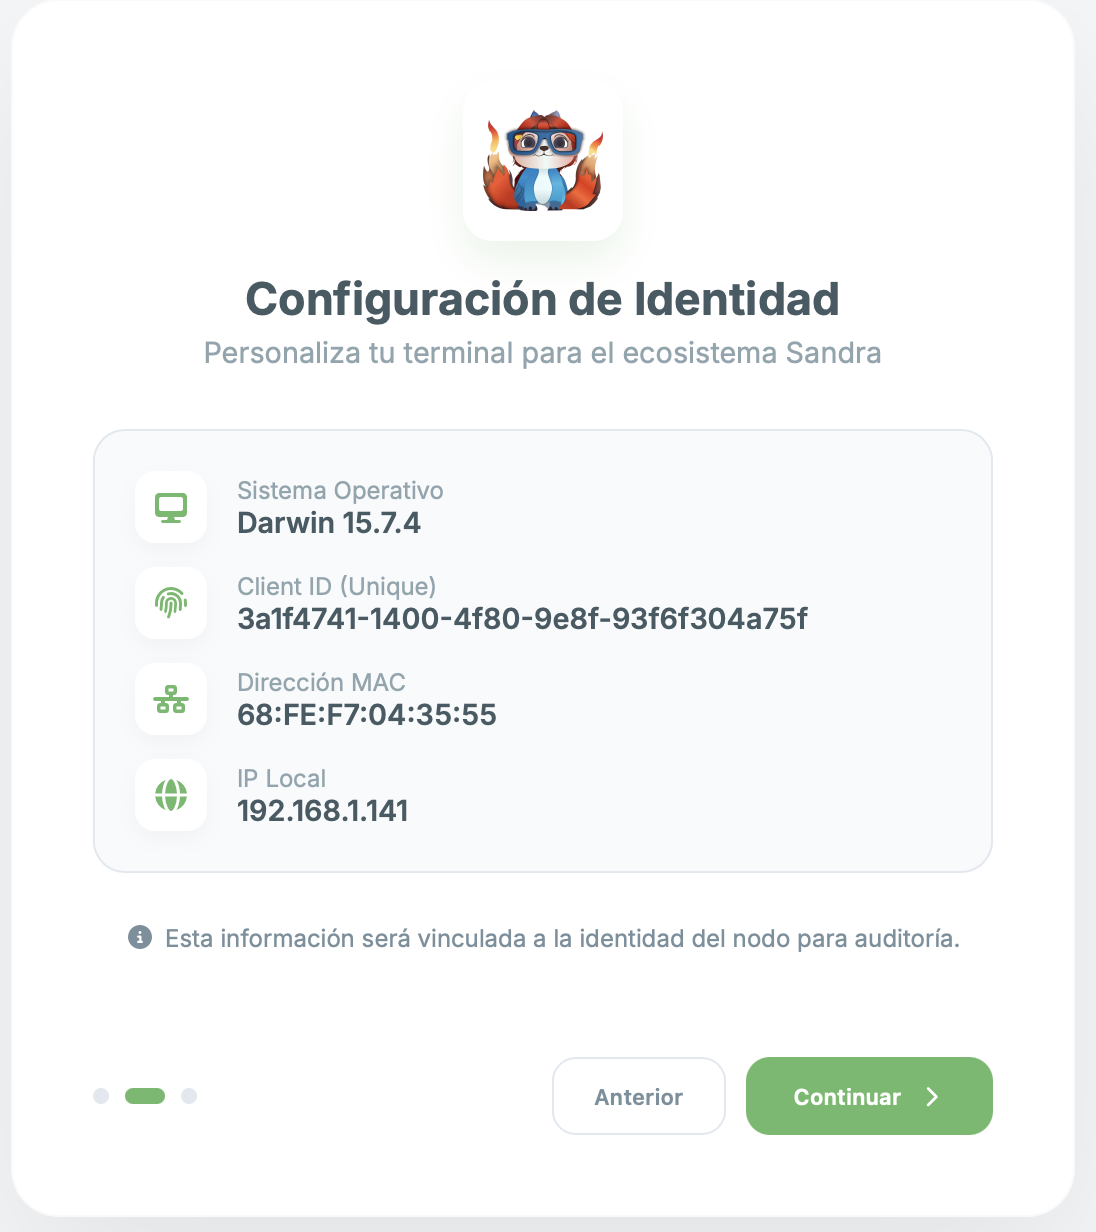
\includegraphics[width=0.3\textwidth]{anexos/3 config.png}
\caption{Vinculacion del nodo}
\label{fig:vinculacion}
\end{figure}

\subsection{Informacion Detectada}

\begin{table}[H]
\centering
\begin{tabular}{p{4cm}p{3cm}p{7cm}}
\toprule
\textbf{Parametro} & \textbf{Ejemplo} & \textbf{Uso} \\
\midrule
Sistema Operativo & Darwin & Compatibilidad \\
IP Local & 192.168.1.100 & Registro \\
MAC Address & AA:BB:CC:DD:EE:FF & Identificacion fisica \\
Client ID & UUID v4 & ID criptografico \\
\bottomrule
\end{tabular}
\caption{Informacion detectada}
\label{tab:info-entorno}
\end{table}

\begin{infobox}[Firma Digital]
El Client ID firma todas las operaciones para auditoria.
\end{infobox}

\section{Pantalla de Bienvenida}

\begin{figure}[H]
\centering
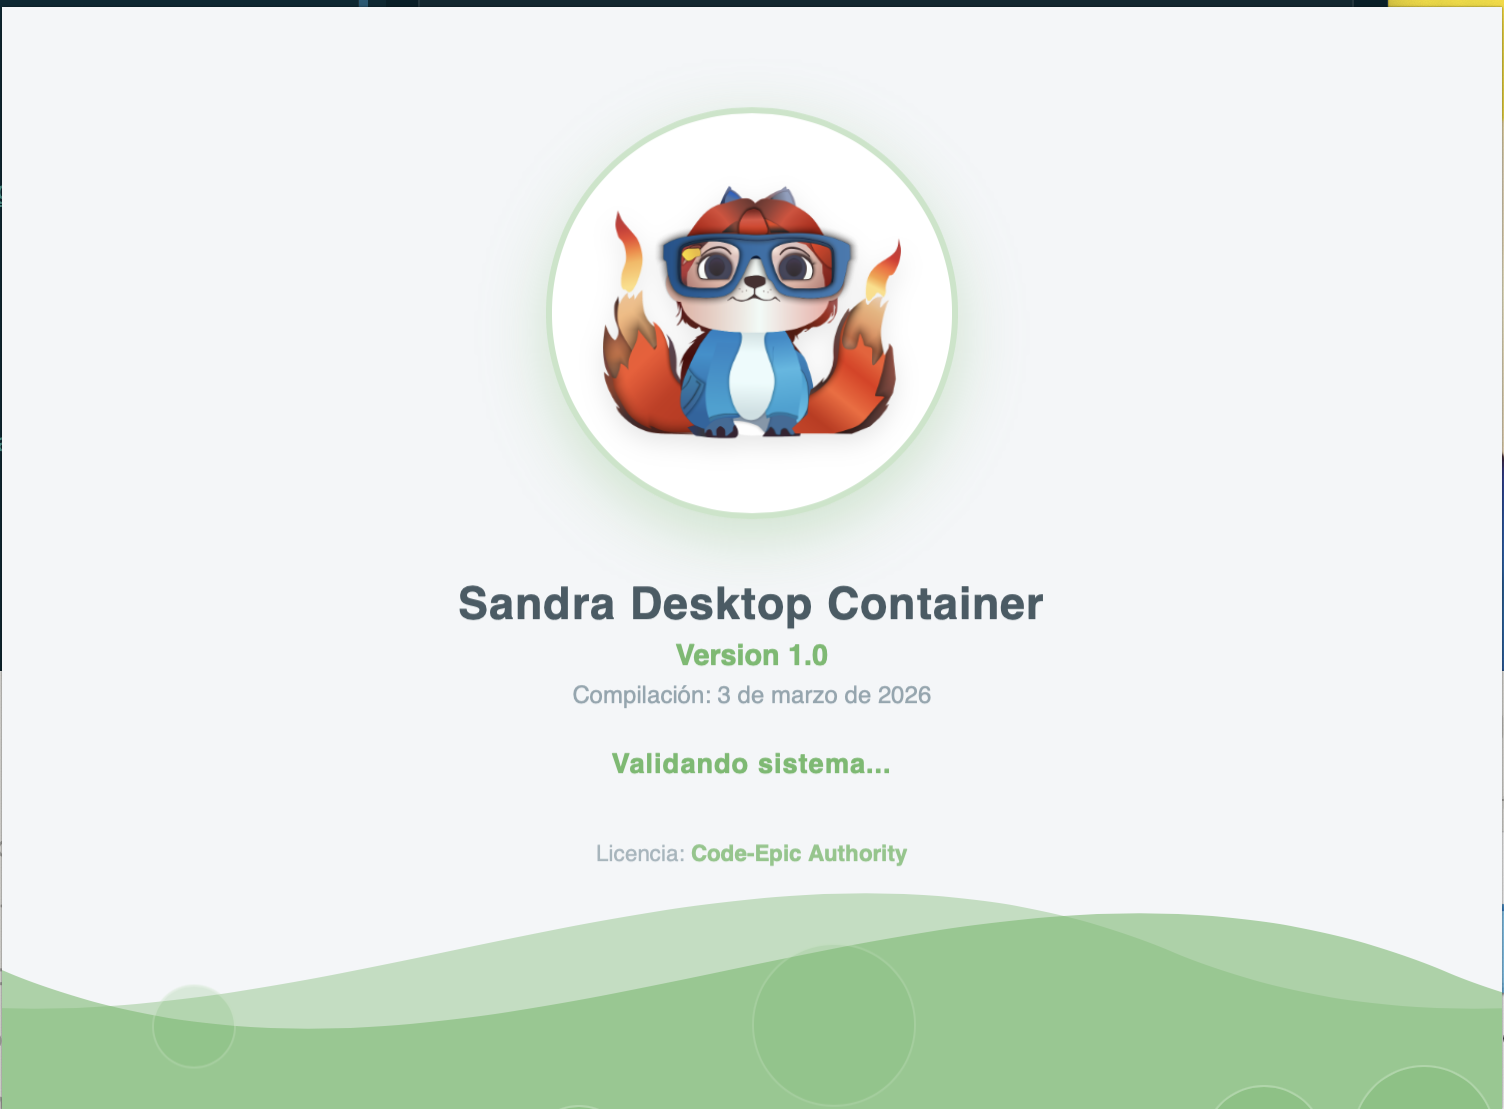
\includegraphics[width=0.9\textwidth]{anexos/1 splash.png}
\caption{Splash screen}
\label{fig:splash}
\end{figure}
